\chapter{Mathematical Foundations of Neural Networks} \label{ch:math-behid}

Understanding the mathematical foundations of the deep neural network is important for searching suitable network architecture. The approach of implementing a model without understanding the mathematical foundation could lead to unexpected failure in getting the desired results from the model. Understanding fundamental mathematics of \acl{AI} is necessary as further development in this field is on going.   \parencite{Kutyniok.16032022} states two different research direction intersects with mathematics and \acl{AI}. One which place the network architecture and training process on theory of mathematics and another with a goal to develop  mathematical problem settings such as partial derivatives equations aiming to tap the potentials of neural network.

Often it is said that an artificial neural network mimics the structure of a biological brain. As illustrated in figure \ref{fig:bio neuron}, a brain is a deep network of neurons which processes the input signals received from Dendrites and transited with Axon. Before transmitting these incoming signals are integrated or summed together in some way and if resulting signal exceeds some threshold then the neuron will transmit it to other neurons.   
\begin{figure}[H]
    \centering    
    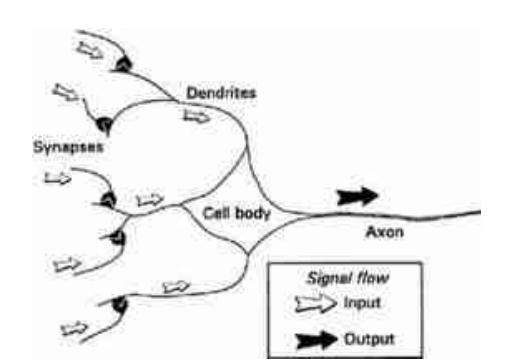
\includegraphics[scale=0.4]{bio_neuron.png}
    \caption{Component of biological neuron in stylized form \parencite[section 1.1]{Gevin.1997}}
    \label{fig:bio neuron}
\end{figure}

The artificial equivalent of a biological neuron is shown in figure  \ref{fig:basic neuron}. The Synapses of figure \ref{fig:bio neuron} are modelled as number or weight being multiplied to each input signals. The weighted signals are summed together by simple arithmetic addition. The resulting value is passed though an activation function representing threshold logic units \parencite[section 1.1]{Gevin.1997}.

\section{Neural Networks and Loss Minimization}

\subsection*{Neurons}

A neural network is a connection of neurons. A Neuron takes input, do some computation and returns an output.  Figure \ref{fig:basic neuron} illustrates a example of   basic unit of neuron, which is multiplying each unit of inputs with weight $w$ and weighted input are added with bias $b$. Finally, the sum is passed though a activation function $ f $.   
\begin{figure}[H]
    \centering    
    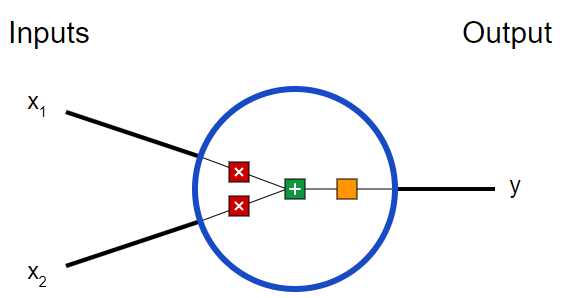
\includegraphics[scale=0.4]{neuron.png}
    \caption{Basic unit of Neuron \parencite{VictorZhou}}
    \label{fig:basic neuron}
\end{figure}


\begin{align}
    y = f(x_1 * w_1 + x_2 * w_2 + b) \label{eq:single_n}
\end{align}

The equation \ref{eq:single_n} is the mathematical representation of the sample neuron. The artificial neurons can be added and concatenated into new functions eventually leading to a complex function. A neuron's characteristics is determined by its parameters and activation functions. Each of the activation functions have a mathematical particularity and their practical effects \parencite{Lederer.25012021}. 

\subsection*{Neural Network}


% \begin{align}
% {\displaystyle \sigma (x)\doteq {\frac {1}{1+e^{-x}}}}$ \label{eg:sigmoid}
% \end{align}



\begin{figure}[H]
    \centering

    % Define block styles
\tikzstyle{input} = [draw, circle, minimum width=0.5cm, minimum height=0.5cm, text centered, text width=1cm, fill=blue!20]
\tikzstyle{hidden} = [draw, circle, minimum width=0.5cm, minimum height=0.5cm, text centered, text width=0.5cm, fill=green!20]
\tikzstyle{output} = [draw, circle, minimum width=0.5cm, minimum height=0.5cm, text centered, text width=0.5cm, fill=red!20]
\tikzstyle{arrow} = [thick,->,>=stealth]

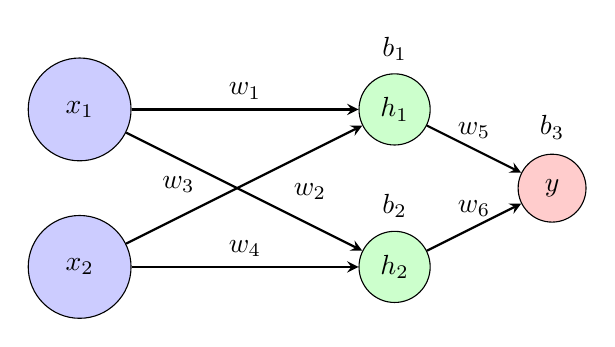
\begin{tikzpicture}[node distance=2cm]

% Input layer
\node (input1) [input] {$x_1$};
\node (input2) [input, below of=input1] {$x_2$};

% Hidden layer 1
\node (hidden1) [hidden, right of=input1, xshift=2cm] {$ h_1 $};
\node (hidden2) [hidden, below of=hidden1] {$ h_2 $};
\node [above=0.5cm] at (hidden1) {$ b_1 $} ;
\node [above=0.5cm] at (hidden2) {$ b_2 $} ;





% Output layer
\node (output) [output, right of=hidden1, yshift=-1cm] {$ y $};
\node [above=0.5cm] at (output) {$ b_3 $} ;
% Arrows
\draw [arrow] (input1) -- node[above] {$w_1$} (hidden1);
\draw [arrow] (input1) -- node[above, right=0.5cm ] {$w_2$} (hidden2);
\draw [arrow] (input2) -- node[above, left=0.5cm ] {$w_3$} (hidden1);
\draw [arrow] (input2) -- node[above] {$w_4$} (hidden2);
\draw [arrow] (hidden1) -- node[above] {$w_5$} (output);
\draw [arrow] (hidden2) -- node[above] {$w_6$} (output);



\end{tikzpicture}
\caption{Example of feedforward neural network: two neuron hidden layer added between input and output.}
   \label{fig:nn_hl} 
\end{figure}

Figure \ref{fig:nn_hl}, illustrates addition of two neurons hidden layers $h_1$ and $h_2$ between input layer (first) and output layer (last). The data flow is represented with directed arrows, this process of passing input forward to get an output is called feed-forward. A feedforward neural network comprises many functions associated with a \acl{DAG}. These chain of functions form a deep layers of the network and such is the term deep learning being tossed  \parencite[chapter 6]{Goodfellow-et-al-2016}.

\subsection*{Training a Network}

Training a network simply means to compare the actual machine learned output ($ y_{ml} $) and correct or true output ($ y_ {true} $) at each time step and determine how good it is at the current time step and what to do to make it better in next time step. Loss function ($ L $) is a way to determine it. 

Let us use the network of figure \ref{fig:nn_hl} to predict the gender based on weight and height. $x_1$ is weight and $x_2$ is height. Table \ref{table:Sample Training Dataset} is a sample of dataset, genders are valued as 0 and 1. The numerical values of height and weight are adjusted to for easier calculation. 

\begin{table}[h]
    \centering
    \caption{Sample Training Dataset}
    \label{table:Sample Training Dataset}
    \begin{tabular}{ llll }
          \toprule
          
          \textbf{Name}& \textbf{Weight} & \textbf{Height}  & \textbf{Gender}\\
          \midrule
          Mary&-2 & -1 & 1\\
          John&25 & 6 & 0\\         
         
          \bottomrule
          \end{tabular}
\end{table}


Equation \ref{eq:MSE} is \acf{MSE} which is one loss functions. 
\begin{align}
    \text{MSE} = \frac{1}{n} \sum_{i=1}^{n} (y_ {true} - y_{ml})^2 \label{eq:MSE}
\end{align}


\begin{itemize}
    \item $n$ is a number of samples. In table \ref{table:Sample Training Dataset} there are two entities.
    \item $y$ is the value the machine needs to generate, in this case ``Gender''.
    \item $y_ {true}$ is the correct value, for name ``Mary'' the correct gender value is 1. $y_ {ml}$ is the machine  predicted value.
    \item $(y_ {true} - y_{ml})^2$ is known as squared error. This loss function takes average of the squared error.
\end{itemize}



If the machine always returns the value 0, what is the loss?

\begin{table}[h]
    \centering
    \caption{Sample Training Dataset}
    \label{table:Sample Training Dataset}
    \begin{tabular}{ cccc }
          \toprule
          
          \textbf{Name}& \textbf{$y_ {true}$} & \textbf{$y_ {ml}$}  & \textbf{$(y_ {true} - y_{ml})^2$}\\
          \midrule
          Mary&1 & 0 & 1\\
          John&0 & 0 & 0\\         
         
          \bottomrule
          \end{tabular}
\end{table}

\begin{align}
    \text{MSE} = \frac{1}{2} (1+0)^2 = 0.5
\end{align}

Lower loss indicate the network is trained well. The goal of training is minimizing the loss. 


\subsection*{Minimizing the Loss} \label{sec:minloss}

From equation \ref{eq:single_n} it is known that tweaking weights ($w$) and biases ($b$) changes the output value.  How do we change the networks weights and biases such that the loss is decreased at each time step? Answer to this question is partial derivatives. Partial derivatives is a method of small change in one of the variable of a multivariable function leading to a small change in the output of the function. For example, making a small change in variable $w_1$ keeping all other variables constant leading to a small change in Loss $L$ can be represented by equation \ref{eq:loss_partial}.

\begin{align}
    \frac{\partial L }{\partial w_1} = \frac{\partial L}{\partial y_{ml}} * \frac{\partial y_{ml}}{\partial w_1}
    \label{eq:loss_partial}
\end{align}

Referring to the network architecture of figure \ref{fig:nn_hl} $w_1$ does not affect $h_2$ but only $h_1$, the equation \ref{eq:loss_partial} can be rewritten as equation \ref{eq:backprop}.

\begin{align}
    \frac{\partial y_{ml}}{\partial w_1} = \frac{\partial y_{ml}}{\partial h_{1}} * \frac{\partial h_{1}}{\partial w_1}
    \label{eq:loss_partial2}
\end{align}

\begin{align}
    \frac{\partial L }{\partial w_1} = \frac{\partial L}{\partial y_{ml}} * \frac{\partial y_{ml}}{\partial h_{1}} * \frac{\partial h_{1}}{\partial w_1} \label{eq:backprop}
\end{align}

Calculating partial derivatives by working backwards is known as back propagation. 

The final output of the network can be represented as equation \ref{eq:yml}.

\begin{align}
   y_{ml} = o_1 = f(w_5h_1 + w_6h_2 + b_3)
    \label{eq:yml}
\end{align}

\subsection*{\acf{SGD}}

Optimization problem is to find the value for set of variable that minimizes the scalar-valued loss function \parencite[Page 273]{pml1Book}. \acs{SGD} is an optimization algorithm to change weights and biases at time step $t$. Weight of the next time step ($w_{t+1}$) is calculated by subtracting partial derivatives of Loss function with respect to the weight of current time step ($w_t$).  The constant $l$ represents the step size or learning rate. The resulting equation is given \ref{eq:sgd}.  

\begin{align}
 w_{t+1} = w_{t} - l \frac{\partial L }{\partial w_t} \label{eq:sgd}
\end{align}


\section{Probability Distribution}

A probability distribution is the information of how likely a random variable or set of variables is to take each of its possible states. The way the probability distribution is described depended on whether the variables are discrete or continuous. A discrete random variable has finite or countably infinite number of states. \parencite[Page 54]{Goodfellow-et-al-2016}.  

In this project, the random variables are vector-valued product features denoted as $ \textbf{x} $ and its value as $ x $. The probability that variable $\textbf{x} = x$ is denoted by $ P(x) $, with a probability of 1 indicating that $\textbf{x}-x$ is certain and probability of 0 indicating an impossible event \parencite[Page 55]{Goodfellow-et-al-2016}.


The probability values ranging between 0  and 1 are called \acf{PMF} denoted as capital $ P $. To ensure that \acs*{PMF} provides valid probabilities the function $P$ must satisfy following properties.


\begin{itemize}
    \item Domain of PMF must be defined for all possible states of random variable $x$. It should specify probabilities for each value $x$. For example, of the variable of vector representation of product name ``X'' the $P$ must be defined for all categories.
    \item The $ P(x) $ must satisfy $0 \leq  P(x) \leq  1$.
    \item Impossible events have probability 0.
    \item Certain events have probability 1.
    \item Normalization property indicating sum of all probabilities equals to 1.
\end{itemize}


\begin{table}[H]
    \centering
    \begin{tabular}{ccccccc}
        \hline
        $x$ & $x_1$ & $x_2$ & $x_3$ & $\dots$ & $x_n$ \\
        \hline
        $P(x)$ & $P_1$ & $P_2$ & $P_3$ & $\dots$ & $P_n$ \\
        \hline
    \end{tabular}
    \caption{Probability Distribution $P(x)$ for Random Variable $x$}
    \label{tab:probability-distribution}
\end{table}


where \(P_i > 0\), \(i \equiv 1\) to \(n\) and \(P_1 + P_2 + P_3 + \ldots + P_n = 1\) \\

\subsection*{Multinoulli Distribution or Categorical Distribution}

Multinoulli or Categorical distribution is a type of probability distribution over a single discrete variable with $ k $ different states or categories, where $ k $ is finite and probability of each category is separately specified.

\begin{itemize}
    \item A multinoulli distribution is parametrized by a vector $\mathbf{p} \in [0, 1]^{k-1}$, where each element of $\mathbf{p}$ represents the probability of the $i$-th state. 
    \item  The probability of the final, $k$-th state is given by $1 - \sum_{i=1}^{k-1} p_i$. 
    \item  $\sum_{i=1}^{k-1} p_i \leq 1$ hence, the probabilities do not exceed 1. 
\end{itemize}



Multinoulli distributions are often employed to model distributions over categories of objects. In this context, we do not assume that state 1 has a numerical value of 1, and so forth. The values in $\mathbf{p}$ represent probabilities associated with different categories or states, and they do not carry a numerical interpretation.

Moreover, when working with multinoulli-distributed random variables, it is typically unnecessary to compute expectations or variances since these distributions are used to describe categorical outcomes where numerical operations may not be meaningful \parencite[Page 60,61]{Goodfellow-et-al-2016}. 

\section{Activation Functions and their Propertise}
\subsection{Softmax}

The softmax function is often used to predict the probabilities associated with a multinoulli distribution \parencite[Page 79]{Goodfellow-et-al-2016}.

\begin{align}
    \text{Softmax}(x_i) = \frac{{\exp(x_i)}}{{\sum_{j=1}^n \exp(x_j)}} \label{eq:softmax_matth}
\end{align}

Equation \ref{eq:softmax_matth} is the formula for Softmax function. It applies the standard exponential function to each element $ x_i $ of the input vector $ \mathbf{x} $  and normalizes these values by dividing by the sum of all these exponential. 

\begin{lstlisting}[language=Python,caption={Python example for softmax},label=code:sample_softmax]
    >>> import numpy as np
    >>> a = [1.0, 2.0, 3.0, 4.0, 1.0, 2.0, 3.0]
    >>> np.exp(a) / np.sum(np.exp(a))
    array([0.02364054, 0.06426166, 0.1746813 , 0.474833  , 0.02364054,
           0.06426166, 0.1746813 ])
    >>> sm_val =np.exp(a) / np.sum(np.exp(a))
    >>> np.sum(sm_val)
    0.9999999999999999
    >>>
\end{lstlisting}

Listing \ref{code:sample_softmax} is an example of applying Softmax function to an array of positive integers. It is important to note that the sum of all the softmax value is approximately equal to 1.  The output has most of its weight where the ``4'' was in the original input. This is what the function is normally used for: to highlight the largest values and suppress values which are significantly below the maximum value.



\subsection*{Reasons to apply log to $SoftMax$ function} \label{sec:Logsoft}

 
\begin{align}
    \log(\text{Softmax}(x_i)) = \log\left(\frac{{\exp(x_i)}}{{\sum_{j=1}^n \exp(x_j)}}\right) \label{eq:log_softmax}
\end{align}

Equation \eqref{eq:log_softmax} shows the logarithm of the Softmax function applied to the element \(x_i\) in the vector \(\mathbf{x}\). 

Applying logarithm to the fraction: 
\begin{align}
    \log\left(\frac{a}{b}\right) = \log(a) - \log(b)
\end{align}

Substituting \(a = \exp(x_i)\) and \(b = \sum_{j=1}^n \exp(x_j)\) in equation \eqref{eq:log_softmax}, we get:

\begin{align}
    \log(\text{Softmax}(x_i)) = \log(\exp(x_i)) - \log\left(\sum_{j=1}^n \exp(x_j)\right)
\end{align}

\begin{itemize}
    \item Reduce large numbers:  The softmax function normalizes any value from [-infy, +infy] by applying an exponential function. Exponential functions can lead to a very large numbers, resulting in  Nan as output. Applying logarithm effectively reduce these large numbers to manageable range.
    \item Numerical Stability: When dealing with very small probabilities, the product of multiple probabilities can become exceedingly close to zero, leading to numerical underflow. Similarly, when dealing with very large probabilities, the product can exceed the representation range of standard floating-point numbers, causing numerical overflow. By taking the logarithm, these issues are avoided, and the values are represented in a more stable and manageable range \parencite[Page 79]{Goodfellow-et-al-2016}.
    
    \item Log Probabilities and Addition: Log probabilities are additive when events are independent.\\ For example, if we have two independent events \(A\) and \(B\) with probabilities \(P(A) = p\) and \(P(B) = q\), the probability of both events occurring (\(P(A \cap B)\)) is \(P(A) \times P(B) = p \times q\). Taking the logarithm, we get \(\log(P(A \cap B)) = \log(p \times q) = \log(p) + \log(q)\). This additive property simplifies calculations involving multiple independent events.

    \item Logarithms and Multiplication: Logarithms convert multiplication to addition. Probabilities of independent events,  represented as \(P(A \cap B \cap C \cap \ldots)\). Logarithm of the product of these probabilities simplifies the computation to a sum. 
\end{itemize}

\subsection{Sigmoid or Logistic}

Sigmoid function, also termed as squashing function as the values are bounded in an interval.  Figure \ref{fig:SigmoidActivation} shows the graph of a sigmoid function showing a smooth ``S'' shaped curve. This function is denoted with greek letter $\sigma$ (sigma) and is defined as \parencite[section 2.1]{Lederer.25012021}: 

\begin{align}
    \sigma(x) = \frac{1}{1+ e^{-x}} \label{eq:sigma}
\end{align}

\begin{itemize}
    \item If $x$ to the sigmoid function is a small negative number, the output is very close to 0.
    \item If $x$ is a large positive number, then the output is very close to 1.
    \item If $x$ is 0, the output is $0.5$.
    \item Types of sigmoid functions are logistics, artan, tanh and softsign.
\end{itemize}

\subsection{ReLU Rectified Linear Unit}
In electrical engineering, a rectifier is a device that converts alternating current to direct current. Similarly, this function lets positive inputs pass unaltered but cuts negative inputs as shown in figure  \ref{fig:ReLUActivation}. Limitations of ReLU is dying-relu phenomina, which is similar to vanishing gradient decent. The solution to it is leaky-ReLu  \parencite[section 2.2.2]{Lederer.25012021}. 

\begin{figure}[htbp]
    \centering
    \begin{subfigure}{0.45\textwidth}
        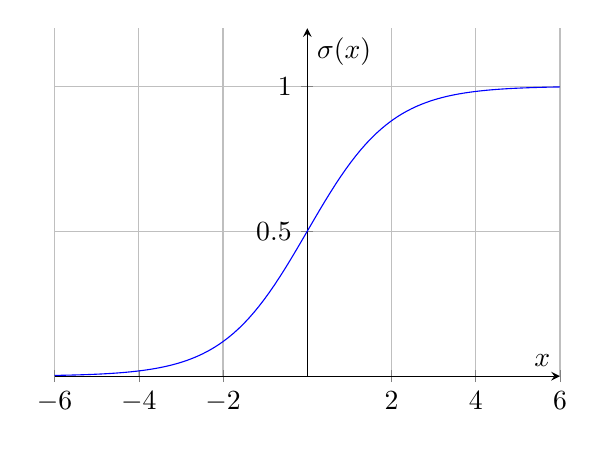
\begin{tikzpicture}
            \begin{axis}[
                xlabel=$x$,
                ylabel=$\sigma(x)$,
                xmin=-6,
                xmax=6,
                ymin=0,
                ymax=1.2,
                width=8cm,
                height=6cm,
                grid=both,
                axis lines=middle
            ]
            \addplot[blue, domain=-6:6, samples=100] {1 / (1 + exp(-x))};
            \end{axis}
        \end{tikzpicture}
        \caption{Sigmoid activation function}
        \label{fig:SigmoidActivation}
    \end{subfigure}
    \hspace{0.05\textwidth}
    \begin{subfigure}{0.45\textwidth}
        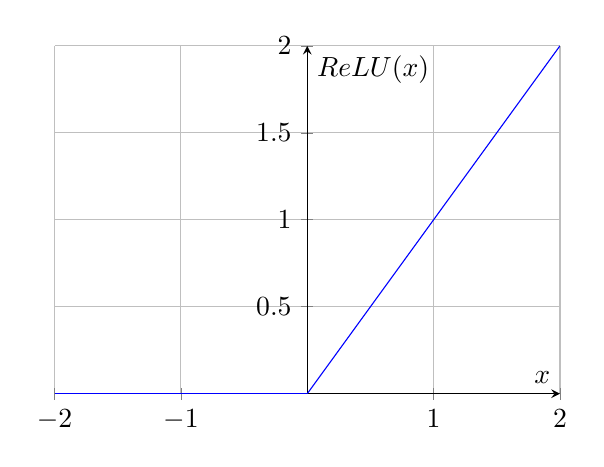
\begin{tikzpicture}
            \begin{axis}[
                xlabel=$x$,
                ylabel=$\text{ReLU}(x)$,
                xmin=-2,
                xmax=2,
                ymin=0,
                ymax=2,
                width=8cm,
                height=6cm,
                grid=both,
                axis lines=middle
            ]
            \addplot[blue, domain=-2:0, samples=100] {0};
            \addplot[blue, domain=0:2, samples=100] {x};
            \end{axis}
        \end{tikzpicture}
        \caption{ReLU activation function}
        \label{fig:ReLUActivation}
    \end{subfigure}
   
    \caption{Activation functions}
    \label{fig:ActivationFunctions}
\end{figure}

\section{ \acs*{RNN} - Forward and Backward Propagation} \label{sec:math-rnn}

When a feedforward neural network are extended to include feedback connections, they are called \acfp{RNN} \parencite[Chapter 6, Page 164]{Goodfellow-et-al-2016}. \acfp{RNN} is best suited for machine learning problems that involve sequential data such as sequence translation, generation and classification. A recurrent neural network is specialized for processing sequence of values $ x^{(1)},\ldots,x^{(t)}$. The prediction of output $y^t$ also depends on the hidden state of the system $h^t$, which gets updated overtime as the sequence is processed \parencite[Chapter 15, Page 501]{pml1Book}.

\begin{figure}[H]
    \centering    
    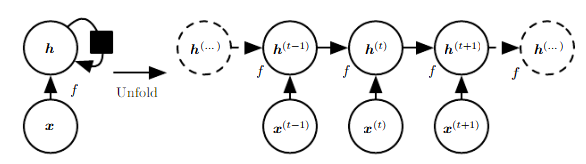
\includegraphics[scale=0.9]{rnn_wno.png}
    \caption{A \acl*{RNN} with no output \parencite[Page 370]{Goodfellow-et-al-2016}}
    \label{fig:RNN without output}
\end{figure}


Figure \ref{fig:RNN without output} illustrates the connected hidden units indicating the output of previous hidden state $h_{(t-1)}$ is the input of current hidden state $h_{(t)}$.  The network can be seen as unfolded computational graphs, here each node is associated with one time instance. This machine learning algorithm store information of previous states and holds the memory. 

Equation \ref{eq:rnn} depicts the common representation of RNN to define the hidden units.

\begin{align}
    h^{(t)} = f(h^{(t-1)}, x^{(t)}; \theta) \label{eq:rnn}
 \end{align}



    \subsection*{Graph Un-rolling and Parameter Sharing}
    
    Here graph is referred to as the structure of a set of computations, such as the data flow from input layer to output layer for mapping the loss. Unfolding the equation \ref{eq:rnn} for $t=3$ times, we obtain:
    
    \begin{align}
        h^{(3)} = f(h^{(2)}, x^{(2)}; \theta) = f(f(h^{(1)},x^{(1)}; \theta)) \label{eq:rnn_new}
     \end{align}
    

    The equation \ref{eq:rnn} is recurrent without the external signal $x^{(t)}$. This expression can be represented by \acl{DAG}.  Unfolding this graph results in the sharing of parameters across a network structure.


    \subsection*{Sequence Generation}

    In this type, the output sequence is generated one token at a time. At every step a sample output $y^t$ from the hidden state $h^t$ is again feed back in to the model to get new state $h^{t+1}$ as illustrated in figure \ref{fig:RNN vectoseq}.  This architecture could be applied in image captioning method \parencite[section 15.2.1]{pml1Book}. 


    \begin{figure}[H]
        \centering    
        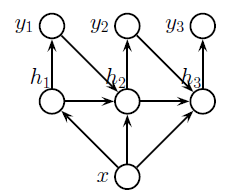
\includegraphics[scale=0.9]{seq_gen.png}
        \caption{A \acl*{RNN} for generating a variable length output sequence given an
        optional fixed length input vector. \parencite[section 15.2.1]{pml1Book}}
        \label{fig:RNN vectoseq}
    \end{figure}

    \subsection*{Sequence Classification}
This architecture take variable length sequence as input and predict an output vector. The output of the hidden state is depended on the previous hidden state and also on input sequence as shown in figure \ref{fig:RNN seqtovec}.
    \begin{figure}[H]
        \centering    
        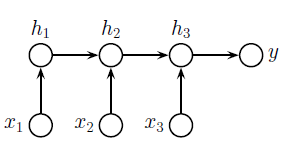
\includegraphics[scale=0.9]{seq_class.png}
        \caption{A \acs*{RNN} for classification \parencite[section 15.2.1]{pml1Book}}
        \label{fig:RNN seqtovec}
    \end{figure}



    \subsection*{Sequence Translation}
There are two types, one in which the input and output are of same length (aligned) and other in which input and output sequence are of variable length(unaligned). 
Application of unaligned sequence translation is machine translation.     
    
    






\section{Summary}

In this chapter, the mathematical theories on neural network is described. Author illustrates mathematical equation for feedforward computational graphs and back propagation. Some mathematical concepts such as partial differentials to calculate the effect of small change in any one of the variable of a neural network is explained with step by step equation. Author describes the using sigmoid, softmax activation function in the output layer of neural network to bound the output values. In this chapter, author explains the \acl{MSE} loss function with a sample of training data. Author discusses the approach for numerical stability to avoid overflow and underflow of value resulting into a not-a-number values.

Further, the author describes multi level classification task.  In this chapter, an overview of the Probability Distribution and one of its type Multinoulli Distribution is given. Author describes the basic architecture of a \acl{RNN} and explains the reason of using this network for categorizing the products based on product name.  